%   % !TEX root = ../../VIII,3_Rahmen-TeX_9-0.tex
%  
%   Signatur/Tex-Datei:	LH_37_05_193
%				
%   RK-Nr. 	57279
%							
%   Überschrift: 	(keine)
%   Titel: 			De regula concursus corporum inaequalium
%   Datierung: 		Januar 1678 (a. St.) VOR "de corporum concursu Scheda 8", eigh.
%   edlabels:	 		4
%   Diagramme: 		2
%
%
\selectlanguage{ngerman}
\frenchspacing
%
\begin{ledgroupsized}[r]{120mm}
\footnotesize
\pstart
\noindent\textbf{Überlieferung:}
\pend
\end{ledgroupsized}
%
\begin{ledgroupsized}[r]{114mm}
\footnotesize
\pstart \parindent -6mm
\makebox[6mm][l]{\textit{L}}%
Konzept:
LH~XXXVII~5 Bl.~193. %ggf. (unsere Druckvorlage).
Ein Blatt~4\textsuperscript{o};
Wasserzeichenfragment am Blattrand;
Papiererhaltungsmaßnahmen;
Ränder beschnitten.
Eine Seite auf Bl.~193~r\textsuperscript{o}; Bl.~193~v\textsuperscript{o} leer.
\pend
\end{ledgroupsized}
%
\begin{ledgroupsized}[r]{114mm}
\footnotesize
\pstart
\parindent -6mm
\makebox[6mm][l]{\textit{E}}%
(tlw.) \textsc{Fichant} 1994, S.~406\textendash408\cite{01056}.
\pend%
\end{ledgroupsized}
%
%
\vspace{5mm}
\begin{ledgroup}
\footnotesize
\pstart
\noindent%
\textbf{Datierungsgründe:}
Leibniz hat das vorliegende Konzept eigenhändig auf Januar 1678 (a.~St.) datiert. 
%
Die folgenden Umstände ermöglichen eine genauere Einkreisung der Entstehungzeit.
%
\pend
%
\pstart
%
In N.~\ref{RK57279} setzt Leibniz die \textit{vis} der Körper mit ihrer Bewegungsgröße bzw.\ dem Impuls gleich, was in der Passage auf S.~\refpassage{37_05_193_4a}{37_05_193_4b} besonders deutlich wird.
%
In den letzten drei Abschnitten von \textit{De corporum concursu}, die eigenhändig auf Januar und Februar 1678 datiert sind, geht Leibniz zu seinem neuen, quadratischen Kraftmaß ($mv^2$) über und nimmt ausdrücklich Abstand von der \textit{quantitas motus} ($mv$). Am deutlichsten geschieht dies in der \textit{Scheda octava} von Januar 1678 
%
(siehe S.~\refpassage{LH_37_05_086r_quadrataceleritatum-1}{LH_37_05_086r_quadrataceleritatum-2} von N.~\ref{dcc_08}), 
%
die deshalb als Terminus ante quem für die Entstehung von N.~\ref{RK57279} gelten darf.
%
\pend
%
\pstart
In seinem
\cite{02053}Brief vom 3.\ (13.) Januar 1678 
gesteht Leibniz gegenüber
\protect\index{Namensregister}{\textso{Conring}, Hermann 1606\textendash1681}H.~Conring,
noch keine befriedigende Antwort auf die Frage
nach dem (geraden zentralen) Stoß zweier ungleicher harter Körper gefunden zu haben
%
(\textit{LSB} II, 1 \lbrack2.~Aufl.\rbrack, S.~581.5\textendash7).
%
Der Umstand, dass N.~\ref{RK57279}
ebendiese Frage untersucht, ohne zu einer eindeutigen Lösung zu gelangen,
und damit genau die im Brief an 
\protect\index{Namensregister}{\textso{Conring}, Hermann 1606\textendash1681}Conring
geäußerte Schwierigkeit verkörpert,
lässt eine Entstehung des Konzepts etwa gleichzeitig zu dem Brief plausibel erscheinen.
%
\pend 
\end{ledgroup}
%
\selectlanguage{latin}
\frenchspacing
%
% \newpage%
\vspace{8mm}
\pstart%
\normalsize%
\noindent%
\lbrack 193~r\textsuperscript{o}\rbrack\
\pend
%
\pstart \noindent
\edlabel{37_05_193_1a}%
\edtext{}{% NEUER ABSATZ UND VARIANTEN "Januar."
{\xxref%
{37_05_193_1a}{37_05_193_1b}}%
\lemma{Januar.}%
\Bfootnote{%
\textit{(1)}~1677 %
\textit{(2)}~1678 %
\textit{(a)}~Non dubit %
\textit{(b)}~Credibile est in %
\textit{(aa)}~motu %
\textit{(bb)}~corporum %
\textit{L}}}%
\raggedleft
Januar. 1678
\pend
%
\pstart \noindent
Credibile est in corporum%
\edlabel{37_05_193_1b}
%
durorum aequalium%
\protect\index{Sachverzeichnis}{corpora dura aequalia} %
concursu illud evenire, 
%
\edtext{quod alii egregii viri dixere.}{\lemma{quod alii egregii viri dixere}%
\Cfootnote{%
\protect\index{Namensregister}{\textso{Wallis} (Wallisius), John 1616\textendash1703}\textsc{J.~Wallis}, \cite{01065}\glqq A summary account \lbrack...\rbrack\ of the general laws of motion\grqq, \cite{00158}\textit{PT} III (1668\textendash1669), Januar 1669, S.~864\textendash866;
%
\protect\index{Namensregister}{\textso{Wallis} (Wallisius), John 1616\textendash1703}\textsc{Ders.}, \cite{00301}\textit{Mechanica}, London 1670\textendash1671, Pars~III, Cap.~XI, Prop.~I und Scholium, S.~660\textendash662 (\cite{01008}\textit{WO} I, S.~1002f.) sowie Prop.~XI, S.~672 (\cite{01008}\textit{WO} I, S.~1009);
%
\protect\index{Namensregister}{\textso{Huygens} (Hugenius, Ugenius, Hugens, Huguens), Christiaan 1629\textendash1695}\textsc{C.~Huygens}, \cite{00529}\glqq Regles du mouvement dans la rencontre des corps\grqq, \cite{00157}\textit{JS} (Pariser Ausgabe), 18.~März 1669, S.~22\textendash24 (\cite{00113}\textit{HO} XVI, S.~179\textendash181), bes.~§§1\textendash2;
%
\protect\index{Namensregister}{\textso{Mariotte}, Edme, Seigneur de Chazeuil ca. 1620\textendash1684}
\textsc{E.~Mariotte}, \cite{00311}\textit{Traité de la percussion}, Paris 1673, Première Partie, Prop.~XV\textendash XVII, S.~90\textendash112.}} 
%
Nam eadem pariter vis,%
\protect\index{Sachverzeichnis}{vis} %
et in summa directio%
\protect\index{Sachverzeichnis}{directio} %
servatur; et fit permutatio velocitatum%
\protect\index{Sachverzeichnis}{permutatio velocitatum} %
pariter ac directionum.%
\protect\index{Sachverzeichnis}{permutatio directionum} %
Sed in corporibus inaequalibus%
\protect\index{Sachverzeichnis}{corpora inaequalia} 
non aeque servari potest regula illa.
\pend
%
%
\vspace{2.0em} %Diagramm Fig. 1
\centerline{%
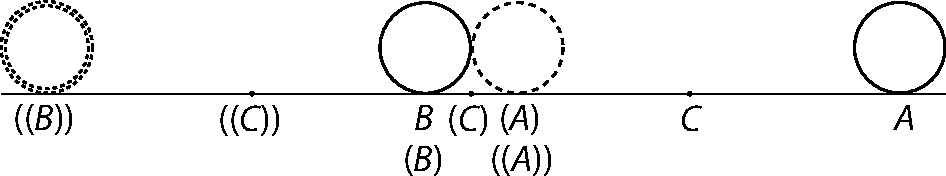
\includegraphics[width=0.7\textwidth]{%
gesamttex/edit_VIII,3/images/LH_37_05_193_d1.pdf%
}} 
\vspace{0.5em}
\centerline{%
\lbrack\textit{Fig.~1}\rbrack%
}
% \newpage%
\vspace{1.5em}%
\centerline{% Diagramm Fig. 2
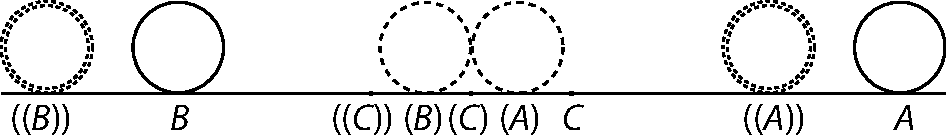
\includegraphics[width=0.7\textwidth]{%
gesamttex/edit_VIII,3/images/LH_37_05_193_d2.pdf%
}} 
\vspace{0.5em}
\centerline{%
\lbrack\textit{Fig.~2}\rbrack%
}
% \newpage%
\vspace{1.5em}
%
%
\pstart
Corpus \textit{A} vocetur \textit{a}, et corpus \textit{B} vocetur \textit{b}. 
Celeritas prioris \textit{e}, posterioris \textit{i}.
\edlabel{37_05_193_4a}%	Zw. Referenzierung
Vis\protect\index{Sachverzeichnis}{vis} prioris \textit{ae}, posterioris $+bi$, summa
%
\edtext{virium\protect\index{Sachverzeichnis}{summa virium} ob contrarium motum $ae-bi$}{\lemma{virium}\Bfootnote{\textit{(1)}~$ae+bi$ \textit{(2)}~ob contrarium motum $ae-bi$~\textit{L}}},%
\edlabel{37_05_193_4b}
%
quae debet manere ante et post concursum.
Haec regula est infallibilis:%
\protect\index{Sachverzeichnis}{regula infallibilis}
%
\rule[0cm]{0mm}{16pt}\textit{AB} aequ.\ $e+i$
%
et
%
$\displaystyle\frac{BC}{AC}$ aequ.\ $\displaystyle\frac{a}{b}$. 
\textit{AB} aequ.\ $BC+AC$. 
\rule[0cm]{0mm}{18pt}Ergo
$BC \ \sqcap \ \displaystyle\frac{a}{b}\,AC$ aequ.\ 
%
\edtext{$AB-AC$. Ergo}{%
\lemma{}%
\Bfootnote{%
$AB-AC$. \textbar\ Ergo \textit{streicht Hrsg.}\ \textbar\ %
Ergo~\textit{L}}}
$AC \ \sqcap \ AB \ \smallfrown \ \displaystyle\frac{1}{1+\displaystyle\frac{a}{b}} \ \sqcap \ \displaystyle\frac{b}{a+b} \ \smallfrown \ e+i$ 
et 
$BC \ \sqcap \displaystyle\frac{a}{a+b} \ \smallfrown \ e+i$
ubi nota literas \textit{a}, \textit{b} semper esse valores positivos, sed \textit{e} vel \textit{i} aliquando esse posse negativos,
%
\rule[0cm]{0mm}{10pt}imo et nihilo aequales. Quaeritur jam longitudo \textit{C}(\textit{C}) progressus centri gravitatis,%
\protect\index{Sachverzeichnis}{progressus centri gravitatis} nempe
%
(posito corpora in puncto consistere) \textit{A}(\textit{A})
%
\edtext{seu $A(C)}{%
\lemma{}%
\Bfootnote{%
seu \textit{A}(\textit{C}) %
\textit{erg.~L}}}%
-AC$, ponendo corpus \textit{A} esse illud quod
in eandem partem cum centro gravitatis%
\protect\index{Sachverzeichnis}{centrum gravitatis}
%
\edtext{tendit, seu quod ipsum sequitur.}{\lemma{, seu}\Bfootnote{quod ipsum sequitur \textit{erg.}~\textit{L}}}
%
Quod locum habet etiam
cum centrum hoc est in ipso loco concursus,%
\protect\index{Sachverzeichnis}{locus concursus}
%
seu quiescit, nam fingi potest in eo
%
motus infinite parvus.%
\protect\index{Sachverzeichnis}{motus infinite parvus}
%
Ergo \textit{C}(\textit{C}) aequ.\ $A(A) - AC$ 
\rule[0cm]{0mm}{18pt}aequ.\ $e - \overline{\displaystyle\frac{b}{a+b} \ \smallfrown \ e+i}$
vel
aequal.
$\displaystyle\frac{ae+be-be-bi}{a+b}$ aequ.\ $\displaystyle\frac{ae-bi}{a+b}$,
quae etiam aequ.\ (\textit{C})((\textit{C})).
Sed eadem (\textit{C})((\textit{C})) aequ.
%
\rule[0cm]{0mm}{12pt}((\textit{B}))(\textit{B}) seu $((B))(C),,-((B))((C))$, prorsus ut ante, invertendo tantum,
itaque pro ((\textit{B}))(\textit{B}) ponendo $\upsilon$, et pro ((\textit{A}))(\textit{A}) 
%
\rule[0cm]{0mm}{16pt}ponendo $\epsilon$, fiet (\textit{C})((\textit{C}))
aequ.\ 
%
$\displaystyle\frac{b\upsilon\edtext{\lbrack-\rbrack}{%
\lemma{}%
\Bfootnote{%
$+$ %
\textit{L ändert Hrsg.}}}%
a\epsilon}{a+b}$
quae antea aequ.\ $\displaystyle\frac{ae-bi}{a+b}$.
Ergo
$b\upsilon -a\epsilon$ 
%
\edtext{aequ.\ $ae-bi$ at ob vires}{\lemma{aequ.\ $ae-bi$}\Bfootnote{\textit{(1)}~at supra \textit{(2)}~at ob vires~\textit{L}}}
\rule[0cm]{0mm}{10pt}easdem 
$ae+bi$ aequ.\ $a\epsilon+b\upsilon $.
Ergo $ae+bi, +ae-bi$ aequ.\ $a\epsilon+b\upsilon, +b\upsilon -a\epsilon$,
seu \textit{ae} aequ.\ $b\upsilon $.
Et pari jure \textit{bi} aequ.\ $a\epsilon$,
sive $\displaystyle\frac{a}{b}$ aequ.\ 
%
\edtext{$\left[\displaystyle\frac{\upsilon}{e}\right]$}{%
\lemma{}%
\Bfootnote{%
$\displaystyle\frac{e}{\upsilon}$ %
\textit{L ändert Hrsg.}}}
%
sive
%
\edlabel{37_05_193_2a}%
\edtext{}{% C-Footnote "et temporum" in Überschneidung mit B-Footnote
{\xxref%
{37_05_193_2a}{37_05_193_2b}}%
\lemma{celeritates \lbrack...\rbrack\ ratione}%
\Cfootnote{%
Bei dem Zusatz \glqq et temporum\grqq\ handelt es sich wohl um ein Versehen, da ein Vergleich der Geschwindigkeiten gleiche Zeiträume voraussetzt.%
}}%
celeritates diversorum corporum et temporum erunt in reciproca corporum
%
\rule[0cm]{0mm}{10pt}\edtext{ratione.\protect\index{Sachverzeichnis}{ratio reciproca}\edlabel{37_05_193_2b} Sed}{%
\lemma{}%
\Bfootnote{ratione %
\textbar\ id est alterum in alterum %
\textit{(1)}~vim %
\textit{(2)}~\textbar~celeritatem \textit{streicht Hrsg.}~\textbar\ %
transfert \textit{erg. u. gestr.}~\textbar\ %
. Sed~\textit{L}}}
%
hinc sequitur corpus magnum impingens in quantulumcunque quiescere, illique totam suam 
vim\protect\index{Sachverzeichnis}{vis}
%
dare; quod experientiae adversum, regula ergo generaliter non 
%
%
\edlabel{37_05_193_3a}%
\edtext{}{% 
{\xxref%
{37_05_193_3a}{37_05_193_3b}}%
\lemma{procedit.}%
\Bfootnote{%
\textit{(1)}~Quid \textit{(2)}~Quod~\textit{L}}}%
procedit.
\pend
%
\pstart
Quod%
\edlabel{37_05_193_3b}
%
si pro regula sumamus non progressum centri gravitatis,%
\protect\index{Sachverzeichnis}{progressus centri gravitatis}
%
sed eandem manere
%
corporum a se invicem distantiam\protect\index{Sachverzeichnis}{distantia corporum a se invicem}
%
ante et post\lbrack,\rbrack\ investigetur ((\textit{B}))((\textit{A})).
%
Illud quidem certum est priori lege (de progressu centri gravitatis aequabili)%
\protect\index{Sachverzeichnis}{lex de progressu centri gravitatis aequabili}
%
observata eandem necessario observari distantiam ante et post concursum, aequali temporis
%
\edtext{intervallo, si celeritates permutatae}{%
\lemma{intervallo,}%
\Bfootnote{%
\textit{(1)}~ob celeritates permutatas %
\textit{(2)}~si celeritates permutatae %
\textit{L}}}
intelligantur, item si navi%
\protect\index{Sachverzeichnis}{navis}
%
utamur motumque compositione\protect\index{Sachverzeichnis}{compositio motuum}
%
explicemus.
\pend\pstart
Sed videndum an non res alia ratione possit
%
\edtext{explicari. Ergo}{%
\lemma{explicari.}%
\Bfootnote{%
\textit{(1)}~Ut %
\textit{(2)}~Ergo %
\textit{L}}}
investigemus\lbrack,\rbrack\ ut dixi, longitudinem ((\textit{A}))((\textit{B})),
%
quod ob casus varios nonnihil 
%
\edtext{intricatum. Obiter}{\lemma{intricatum.}\Bfootnote{\textit{(1)}~Ante omnia \textit{(2)}~Obiter \textit{L}\  }}
%
prius adjicio in priori calculo, supponendo corpora
%
\edtext{non sibi occurrere}{%
\lemma{non}%
\Bfootnote{%
\textit{(1)}~se %
\textit{(2)}~sibi %
\textit{(a)}~exp %
\textit{(b)}~occurrere %
\textit{L}}}
sed \textit{A} sequi \textit{B}, tunc pro 
%
\edtext{\textit{AB} aequ.\ $e+i$}{\lemma{\textit{AB} aequ.}\Bfootnote{\textit{(1)}~$\displaystyle\frac{ae-bi}{a+b}$ nos habituros $ae+bi$ \textit{(2)}~$e+i$~\textit{L}}}
%
nos habituros fuisse $e-i$\lbrack,\rbrack\
ergo \textit{C}(\textit{C}) vel ((\textit{C}))(\textit{C}) aequ.\ 
\rule[0cm]{0mm}{16pt}$\displaystyle\frac{ae+bi}{a+b}$.
\pend \pstart
Unde rursus fiet vel aequ.\ $\displaystyle\frac{b\upsilon +a\epsilon}{a+b}$,
si scil.\ etiam post 
%
occursum\protect\index{Sachverzeichnis}{occursus}
%
ambo prosequitur iter, et orietur tantum 
%
\rule[0cm]{0mm}{10pt}\edtext{aequatio $ae+bi$ aequ.\ $b\upsilon +a\epsilon$ aliunde nota.}{\lemma{aequatio \lbrack...\rbrack\ nota}%
\Cfootnote{%
Siehe bspw.\ N.~\ref{57268} von Mai 1677.}}
\pend
%
%%%%%%%%%%%%%%%%%%%%%%%%%%%%%%%%%
%
\count\Afootins=1200%
\count\Bfootins=1200%
\count\Cfootins=1200